
\title{Hierarchical Controller Architecture in Software Defined Networks}
\author{
        Author 1 \\
            \and
        Author 2\\
        %UIUC\\
			\and
		Author 3\\
}
\date{\today}

\documentclass[10pt, twocolumn]{article}
\usepackage{url,graphicx,tabularx,array,geometry, caption, subcaption, float}
%-- Commands for header
\renewcommand{\title}[1]{\textbf{#1}\\}
\renewcommand{\line}{\begin{tabularx}{\textwidth}{X>{\raggedleft}X}\hline\\\end{tabularx}\\[-0.10cm]}
\newcommand{\leftright}[2]{\begin{tabularx}{\textwidth}{X>{\raggedleft}X}#1%
& #2\\\end{tabularx}\\[-0.10cm]}

\newcolumntype{L}[1]{>{\raggedright\let\newline\\\arraybackslash\hspace{0pt}}m{#1}}
\newcolumntype{C}[1]{>{\centering\let\newline\\\arraybackslash\hspace{0pt}}m{#1}}
\newcolumntype{R}[1]{>{\raggedleft\let\newline\\\arraybackslash\hspace{0pt}}m{#1}}


\begin{document}
\maketitle
\begin{abstract}
Network control plane, in Software Defined Networks (SDN), provides a global view of the physical network to control applications (such as routing), which can be developed as a centralized application rather than a distributed one. Regardless of this abstraction, the control plane itself must inevitably be a distributed system, with multiple nodes called controllers, to achieve desired level of scalability, reliability and responsiveness. 

Traditional architecture involves multiple controllers, each operating on a subset of switches and maintaining a global view of the entire network. We propose a different architecture where controllers are arranged in a hierarchy and only view a part of the network. This improves responsiveness and reduces inconsistency ........(numbers).

Besides, we also propose an optimization in traditional controller architecture. We show 
\end{abstract}

\section{Introduction}
Forwarding or data plane consists of a collection of forwarding elements (switches), connected to form a network, which is inherently distributed in nature. Control plane consists of a collection of control elements, which install forwarding rules on forwarding elements as dictated by control logic or application, running on control elements. Some classes of control applications are routing, traffic engineering (TE), enforcing network policies, etc. In traditional networks, there is a tight coupling and a one to one mapping between control elements and forwarding elements, with one pair on each switch. Besides, the role of control elements had been trivial, which is to merely install instructions given by control application on corresponding forwarding element as forwarding rules. It is the control application which runs distributed protocols to synchronize the state of forwarding elements. The design of these distributed protocols differs from application to application. For example, link state routing makes switches share their neighbors while distance vector routing makes switches share their routing tables.

The emergence of Software Defined Networks (SDN) has induced a separation between forwarding and control elements and has significantly improved the role of the control plane. The control elements may no longer be present on the switches but move to a separate device called a controller, and use predefined protocol such as OpenFlow [openflow-ref], to install forwarding rules. There may be a one-to-many mapping from controllers to switches. At one extreme, control plane may provide a control application with the global network view, which can then be implemented as a centralized application, rather than a distributed one. Regardless of this abstraction, the control plane itself must inevitably be a distributed system, with multiple controllers, to achieve desired level of scalability, reliability and responsiveness.

Conventional control plane architectures involve multiple controllers, where each controller operates on a subset of switches and maintains a global view of the entire network, which is exposed to the control application. Instructions (forwarding rules) from control application are sent to target switches directly or through other controllers. Underlying network state is shared with other controllers through distributed state dissemination frameworks such as distributed transactional databases or Distributed Hash Tables (DHT). Consequently, this introduces a trade-off between network state inconsistency and responsiveness. Results from [logically-centralized-ref] suggests that control state inconsistency significantly degrades performance of logically centralized control applications agnostic to the underlying state distribution.

The state inconsistency problem arises from the fact that each controller tries to maintain the complete global view of the network. Besides, we believe that it is difficult (from scalability point of view) for a controller (a COTS machine) to handle the entire network view. Motivated by these observations, we propose a hierarchical controller architecture. We show ....................   
 

\paragraph{Outline}
The remainder of this article is organized as follows. Section~\ref{sec:hierarchical} presents Hierarchical Controller Architecture. We present the experimental results in section~\ref{sec:eval}. In section~\ref{sec:timestamps}, we present an optimization to conventional controller architecture to help improve the performance of application even if states between controllers is inconsistent. Related work is presented in section~\ref{sec:related}. We discuss ............Our new and exciting results are described in Section~\ref{sec:eval}.


\section{Hierarchical Controller Architecture}
\label{sec:hierarchical}
We propose a new control plane architecture in which controllers are arranged in the form of a tree over the physical network. Switches form the leaf nodes in the tree, while controllers form the internal nodes [TODO:tree-figure]. An internal node acts as a switch for its parent and as a controller for its children. A node aggregates its underlying network and converts it to a switch abstraction which is then exposed to the parent controller. This switch abstraction is explained in detail in section~\ref{subsec:aggr}. A controller's view does not span the whole network but only the network of its children. A node translates instructions (forwarding rules) from its parent controller to the forwarding rules for its underlying network. Similarly, network updates from the underlying network are translated into network updates arising from one switch abstraction of the given controller and are passed on to parent controller. The translation process is explained in the following section.

\subsection{One switch abstraction}
\label{subsec:aggr}

\subsection{An example}
\label{example}
Let's consider an example to understand the benefits of hierarchical architecture. Let there be a TE control application running on $d$ controllers, with each controller operating on $d$ switches. Network state consists of current utilizations of all links. Whenever a new flow arrives, application choses a path with minimum maximum utilization and assigns it to the flow. Each time a path of length $l$ is assigned to the flow, there could be a maximum of $l*d$ link utilization updates and $l$ forwarding rule messages to be sent between controllers. Now, consider an architecture where controllers are arranged in hierarchical manner. There are $d+1$ controllers. The first $d$ controllers (called type 0) maintain $d$ switches each and acts as a switch to the last controller (called type 1), which in turn maintains the other $d$ controllers. Type 0 controllers keep track of link utilizations only for the links that connect it's children switches. Type 1 controller keep track of links that runs from switches belonging to one controller domain to another. Same TE control application runs on each controller. When a new flow arrives, a switch sends $packet_{in}$ message to its type 0 controller. Type 0 controller checks if the path of the flow belongs entirely to its underlying network or not. If yes, it uses TE application to assign the path to the flow and no updates are sent to any controller. However, if the destination is outside its domain, type 0 controller sends a $packet_{in}$ message to its parent controller. Parent controller uses TE control application to assign a paths of type 0 controllers. Forwarding rules are sent to type 0 controllers, which in turn sets up forwarding rules in their network. If the path length is $l$, there will be a maximum of $l+1$ forwarding rule messages between controllers and no link utilization updates. This significant reduction in communication overhead comes at the cost of sub-optimality in the application performance. We show experimentally that the proposed architecture significantly reduces communication overhead while only modestly degrading application performance in the next section.

\section{Evaluation}
\label{sec:eval}
We simulated a dummy control application on both hierarchical as well as flat controller architecture, with same network topology and flow arrival distribution. The details of simulation, metrics and results are presented in this section.

\subsection{Implementation}
\label{sec:implementation}
We wrote our own simulator, which is available at [TODO REF simulator]. We did not use an existing simulator/controller such as Mininet with Floodlight [TODO ref] for the following two reasons: (1) Existing controller lacks the support for flexible controller architecture and are not suitable for hierarchical arrangement of controllers. Modifying existing controllers such as Floodlight to add support for One-switch abstraction (section~\ref{subsec:aggr}), is not a good idea because it requires code/design changes in their primitive modules. Besides, we were not looking for a feature rich controller at that point of time. (2) Existing simulators do not provide controls to regulate replication between controllers or to measure communication overhead (number of messages exchanged ) between controllers, which we needed for evaluation of control plane architecture. Given the above requirements, it seemed easier to write a simulator which provides one-switch abstraction support for the controllers. There are three prime interfaces: (1) {\it Switch Data Plane:} It is implemented by a switch to create forwarding elements to handle packet forwarding according to forwarding rules. (2) {\it Switch Control Plane:} It is implemented by both controllers and switches and is used to establish connections to parent controllers to send packets which do not match any forwarding rule and to receive forwarding rules from parent controller. (3) {\it Controller Control Plane:} It is implemented by controllers to establish connections to children switches/controllers. It is used to receive packets which do not match any forwarding rule and to send forwarding rules to children switches/controllers.Simulator defines two networks: (1) {\t Data Network:} This network consists of all switches (and no controller) connected through links. (2) {\it Management Network:} This network consists of all controllers and switches connected through Controller - Switch Control Plane interfaces. This network allows flexible controller architecture, which could be hierarchical or flat.

To observe the effect of different architecture in real world applications, we used SWIM project [TODO ref swim], which provides synthetic representative test workloads  by sampling historical MapReduce cluster traces using [swim paper ref TODO]. The original trace comes from historical Hadoop traces on a 600 machine cluster at Facebook and spans 6 months, and contains roughly 1 million jobs. The representative trace file contains ~6000 jobs. The trace was simulated with a cluster of 600 machines (as in the original cluster) connected through a network of 200 switches and 10 Gbps links. The cluster is divided into 10 control domains, with 60 hosts, 20 switches and one controller for each domain. Each switch in a domain is connected to 1 to 4 switches within the same domain, with degree being chosen randomly. Each domain contains two Top-of-the-rack switches which inter-connects domains. For hierarchical architecture, there are 11 controllers: 1 controller per domain and one root controllers which manages the other 10 controllers. While flat architecture consists of 10 peer controllers, one or each domain.

Control application is a TE-cum-routing application. When a new flow arrives, control application finds the path with minimum maximum utilization and sets up forwarding rules (based on IP destination and incoming ports) along the path. If multiple such paths exists (which is frequently the case, due to big network), shortest path (in term of number of hops) is chosen. This application runs on each controller in both hierarchical and flat architecture. However, in the hierarchical architecture, the view of application is limited and may consists of controllers or switches as forwarding elements, while in the flat architecture, control application is presented with global view of the network. For simplicity, we have kept network topology as static i.e. links/nodes do not fail and/or created during the simulation. For each Hadoop job, a dummy MapReduce application choses directory, map and reduce nodes randomly in the network, thus, creating a number of flows which are handled by Control application running on controllers. The duration of flow depends on the bytes needed to transfer and assigned rates.            

\subsection{Results}
\label{subsec:results}

\begin{figure}[t]
\centering
\begin{subfigure}{.5\textwidth}
\label{fig:path}
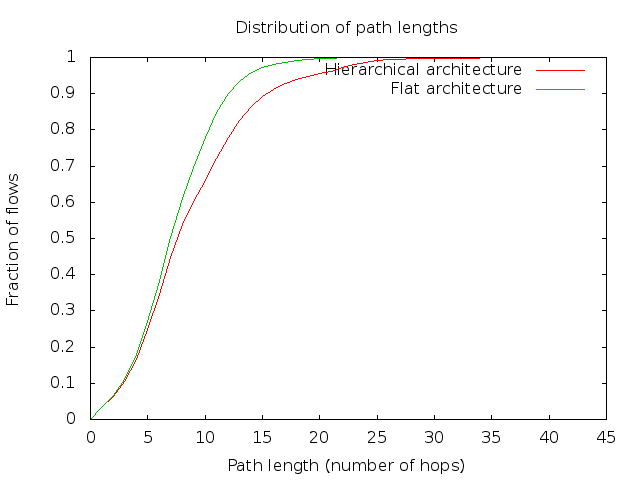
\includegraphics[scale=0.3]{path}
\caption{Application performance: path length for flows}
\end{subfigure}

\begin{subfigure}{.5\textwidth}
\label{fig:util}
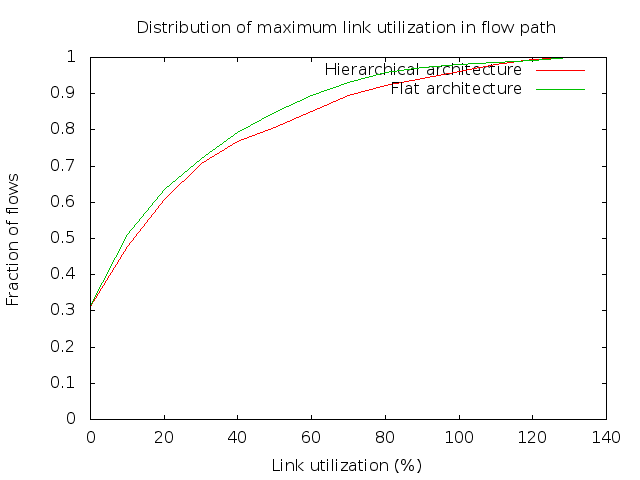
\includegraphics[scale=0.3]{util}
\caption{Application performance: Maximum link utilization for flows}
\end{subfigure}
\caption{Application performance}
\end{figure}

\begin{figure}
\label{fig:msg}
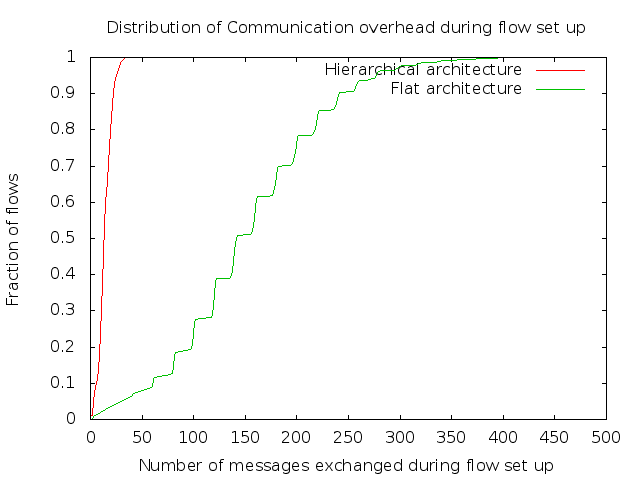
\includegraphics[scale=0.3]{msg}
\caption{Communication overhead per flow}
\end{figure}

We simulated the trace file for both flat and hierarchical architecture, with same topology and same assignment of task nodes for each job. We calculated two metrics: (1) The performance of control application which is measured as the length path (number of hops) assigned to flows (Figure ~\ref{fig:path}) and maximum link utilization encountered by the flow (Figure ~\ref{fig:util}). While the flat architecture gives optimal results, hierarchical architecture provides sub-optimal results. (2) Communication overhead during flow set up, which is measured in term of number of messages passed between switches and controllers as well as within controllers (Figure ~\ref{fig:msg}). The simulation assumes instant replication of network state between controllers. Results show that hierarchical architecture reduces the communication overhead between controllers by an order of magnitude while modestly deviating from optimal solution.

\begin{table*}
\centering
\begin{tabular}{| L{5cm} | L{3cm} | L{3cm} | L{5cm} |}
\hline
& {Average path length} & {Average maximum utilization} & {Average communication overhead per flow} \\ \hline
Flat architecture & 7.81 & 24.62 & 153.54 \\ \hline
Hierarchical architecture & 9.17 & 27.78 & 14.52 \\ \hline
\end{tabular}
\end{table*}%



\section{Timestamps}
\label{sec:timestamps}
We worked hard, and achieved very little.

\section{Discussion}
\label{sec:discuss}

\section{Related Work}
\label{sec:related}
Owing to the performance, reliability and scalability issues faced by single controller architectures, distributed controller architectures have been studied and implemented in various flavors. Most of them aim for a logically centralized global view of the network, while Some of them are discussed in this discussion.

Hyperflow[Hyperflow-ref] has a logically centralized but physically distributed controller architecture. It localizes decision making in individual controllers by passively synchronizing the global network view. The control application is agnostic to the underlying architecture and takes a global decision, though the effect is local. The events are propagated using a publish/subscribe messaging paradigm.

Onix[Onix ref] presents a platform on top of which a network control plane can be implemented as a distributed system. Control planes written within Onix operate on a global view of the network and use basic state distribution primitives provided by the platform. Thus Onix provides a general distributed state management API for control plane implementations, but leaves the decision making and trade-offs among consistency, durability and scalability to the control applications. This makes the design, deployment, modification and verification of control applications difficult and cost prohibitive.

Kandoo[Kandoo-ref] takes a slightly similar approach to our own and presents a two layer hierarchy of controllers: (i) the bottom layer is a group of controllers with no interconnection and no knowledge of the nework-wide state, and (ii) the top layer is a logically centralized controller that maintains network-wide state. Bottom layer runs a local application for its underlying network, while the top layer subscribes to changes from the bottom layer. Top layer view is subscription dependent and the architecture cannot be used in a generic fasion.

On a similar but different note, B4[B4-ref] uses a two level hierarchy, where the site controllers view their local network and aggregate flows to the higher level centralized controller which performs TE. Though the paper talks about a very particular implementation, it demonstrates in practice the benefits of the generic principle of our design.
\section{Conclusion}
\label{sec:conc}

\section{Acknowledgements}
\label{sec:ack}

\bibliographystyle{abbrv}
\bibliography{main}

\end{document} 
